\chapter{Evaluation}
\label{chap:evaluation}
\section{Evaluation}
\label{sec:evaluation}
Given how adverse the Bitcoin community is to change once we evaluate our system we will have to take into account the following factors that are a priority for both Bitcoin users and miners.

\begin{itemize}
\item \textbf{Transaction and block latency} As it was described in the previous section, some of the approaches have an impact on the time it takes to disseminate transactions or blocks. So once we evaluate our system we will have to study if our system does not increase this latency time by a relevant amount. Otherwise, our system might induce more forks on the network which is not desirable.

\item \textbf{Bandwith consumption} This factor is also important for two reasons: i) we want to preserve computational power and ii) we want our system to be scalable.

We want to minimize the number of messages on the network to avoid nodes from wasting computational power processing irrelevant messages. Furthermore, with the growing number of Bitcoin users if our system was to put a big overweight on the network it would not scale well.

Some of our approaches will impose an extra overweight on the network so once we evaluate our system we will have to take into consideration that extra bandwidth and try to minimize it.

\item \textbf{Resources consumption} This is one of the most important factors given the performance requirements imposed by the Bitcoin community. If our system was to downgrade the performance of Bitcoin without a worthy tradeoff our system would never be adopted. It is certain that with the implementation of our approaches the performance aspect of Bitcoin will be affected. So once we evaluate our system we will need to take this into consideration and balance out the performance degradation with the advantages our system brings.
\end{itemize}

Given the complexity of Bitcoin and its dimension we will start by using the Shadow simulator \cite{jansen2011shadow} to evaluate our system. We will use an incremental approach to test our system given the complex system that Bitcoin is. We will start by examining if each our approaches protect Bitcoin against their respective vulnerabilities. Then once we are sure that our strategies work as expected we will combine them together and once again evaluate their effectiveness and also measure the factors presented previously.

Our system should be tested with a workload that contains the same amount of transactions happening these days but the amount of messages should be proportional to the size of the emulated network, for instance, we are not going emulate a system with 10 nodes and 100K transactions.

Finally, once we have a good understanding of the impact Bitshield has in Bitcoin we will generate, if there is still enough time until the deadline of the thesis, a working Bitcoin client ready to be deployed in the network.

Para avaliar a abordagem proposta, construímos um simulador de eventos que modela a propagação de transações na rede Bitcoin (este simulador foi desenvolvido em Python). Decidimos implementar o nosso próprio simulador pois todos os outros que encontrámos não implementavam a versão mais actual do protocolo Bitcoin\footnote{Entre outros \url{https://github.com/shadow/shadow-plugin-bitcoin} e\\ \url{https://github.com/arthurgervais/Bitcoin-Simulator}}.

\subsection{Calibração do Simulador}
\label{sec:calibracao}
De modo a calibrar o simulador para ser o mais fiel possível ao protocolo original, extendemos o \textit{Bitcoin Core}, o cliente Bitcoin mais usado, para recolher métricas relativamente às mensagens trocadas pelos clientes.
As métricas recolhidas são as seguintes: i) anúncios de transações; ii) transações recebidas; iii) transações presentes em blocos compactos que o nó não possuía e tinha de pedir de forma a poder reconstruir o bloco.
Corremos duas instâncias deste cliente, em localizações físicas distintas durante um mês e usámos as métricas recolhidas para calibrar e validar o simulador.
Além disso usámos a informação publicamente disponível em \url{https://blockchain.info/} para determinar o número de transações criadas por dia, a distribuição de blocos gerados por mineiro, e o tamanho médio de uma transação.
Munidos destas métricas, implementámos o protocolo original no simulador, bem como as nossas modificações. Calibrámos experimentalmente o simulador de modo a que os resultados observados no Bitcoin fossem equivalentes às observações efetuadas no cliente real.
O modelo de rede que usámos para as simulações foi composto apenas por nós que seguem o protocolo devidamente.

%As simulações recorrem a simulador de eventos discreto, programado em Python,  que funciona por ciclos. Em cada ciclo os nós verificam se têm eventos para processar e, em caso afirmativo, executam o código que processa esse evento. Este código mimetiza o comportamento de um cliente Bitcoin (foram concretizadas duas versões, uma que tem o comportamento padrão e outra que corre as nossas modificações). Como resultado de processar um evento, um nó pode gerar novos eventos (que serão processados em ciclos futuros). Cada ciclo do simulador corresponde a um segundo de tempo real.




%Para testar a nossa solução corremos o nosso simulador em diferentes maquinas para diferentes tamanhos de rede. Para realizar a maior partes dos testes usamos um computador pessoal com um Intel i5-4590 e 12GB de RAM usamos também para correr testes de maior dimensão uma maquina com um AMD Opteron 6272 e 32GB de RAM e outra maquina com um XX e 125GB de RAM.


%Dados serem computacionalmente dispendiosas, as simulações foram corridas para diferentes tamanhos de rede mantendo o rácio de mineiros observado na data de realização das experiências, 6000 nós para 16 pools de mineiros cada uma com 3 gateways em média. Assim os diferentes tamanhos de rede testados foram: 625 nós com 5 mineiros, 1000 nós com 12 mineiros e 6000 nós com 48 mineiros todos para uma duração equivalente a um dia em tempo real.
Devido às simulações serem computacionalmente dispendiosas e demorarem muito tempo a correr (na ordem dos dias) para redes grandes, fizemos testes preliminares para verificarmos se podíamos diminuir proporcionalmente o tamanho da rede e respectivas propriedades sem comprometer os resultados obtidos.
Para este efeito, corremos o protocolo original com 6000 nós e com 625 nós e comparámos várias métricas, que discutiremos mais adiante.
Os resultados obtidos foram equivalentes para ambos os tamanhos de rede pelo que, no resto desta secção consideramos uma rede de 625 nós.
Este escalonamento proporcional entre 6000 nós (tamanho de rede registado quando começamos as experiências) e 625 nós permitiu-nos explorar mais rapidamente o espaço de soluções e correr várias instâncias de cada teste.
Os resultados apresentados são a média de 3 testes independentes e correspondem a 24 horas de tempo real.

%e 16 \emph{pools} de mineiros cada uma com 3 \gateways em média quer com uma rede de 625 nós e 5 pools cada uma com 1 gateway. Assim todos os nossos testes foram realizados para uma duração equivalente a um dia em tempo real com a configuração para os 625 nós.
%no mundo real o que significa 86400 ciclos no simulador.


%De forma a podermos correr múltiplas simulações de uma só vez escrevemos também um \textit{script} em Bash que nos permitia correr as diferentes experiências múltiplas vezes e até paralelamente caso o máquina em questão tivesse recursos suficientes para o fazer.

\subsection{Impacto da Propagação Enviesada}
\label{sec:evalDiss}
Começámos por explorar o espaço de soluções à procura de compromissos que nos permitam reduzir o consumo de recursos de rede sem ter um impacto negativo nas propriedades dos sistema.
Para ser mais fácil denominar as diferentes experiências realizadas usamos a seguinte notação: \textsl{Mn}, em que n especifica o valor da variável \textsl{tamanho\_m} ; e \textsl{An}, em que n especifica o tamanho da variável \textsl{tamanho\_a} conforme especificado no Algoritmo~\ref{alg:diss}.

%\begin{itemize}
%\item Top n - tamanho da lista de melhores nós;
%\item Rand n - tamanho do conjunto de nós escolhidos ao acaso.
%\end{itemize}

Inicialmente, testámos as combinações de $n={1,2,3,4}$ quer para \textsl{M} quer para \textsl{A}.
Após este conjunto preliminar de experiências, observámos que os resultados para $n={3,4}$ eram praticamente indistinguíveis de $n={1,2}$, com a excepção do número de duplicados que permaneceu perto do obtido na Bitcoin original.
Estes resultados suportam também as medições no cliente real, onde observámos um número médio de duplicados de $3.33$.
Deste modo, para o resto das experiências efectuadas, consideramos somente as combinações:
%Inicialmente para que pudesse-mos  averiguar a eficácia da nossa solução começamos por correr um conjunto de experiências com n igual a 4, 3, 2, 1 quer para Top quer para Rand.
%
%Dos resultados destas experiências pudemos concluir que os valores de n a 4 e 3 ainda eram muito elevados pois obtínhamos os mesmo resultados que com n igual a 2 e 1 só que tínhamos uma percentagem de mensagens de anúncios duplicadas ainda muito próxima à versão base. Desta forma decidimos correr os testes para as seguintes combinações:
%\begin{itemize}
M2\_A2;
M2\_A1;
M2\_A0;
M1\_A1;
M1\_A0.
%\end{itemize}
%\textbf{MM: TODO: esta parte deveria esta na especificação acima.}
Adicionalmente, para cada configuração variámos o valor da variável \textsl{pi}.
%Após termos corrido algumas experiências tivemos a ideia de também adicionar um mecanismo a que chamámos \textit{Early push}, que consiste num nó quando cria uma transação em vez de enviar só para o Top e os Rand envia para todos os seus vizinhos. Assim as experiências que vamos observar têm as 5 diferentes combinações e para cada uma ainda mostramos os resultados com o \textit{Early push} ativado e desativado.
Nos dados apresentados abaixo descartámos também a primeira e a última hora de simulação de forma a podermos estudar o sistema em estado estável.
\vspace{-0.7cm}

\begin{figure}
\centering
%\begin{subfigure}{.45\textwidth}
%  	\centering
%	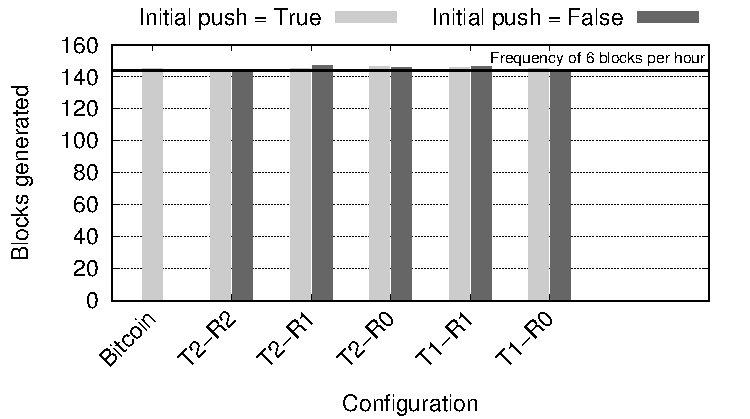
\includegraphics[width=1\textwidth]{plots/blocks-gen.pdf}
\subfloat[Quantidade de blocos criados.]{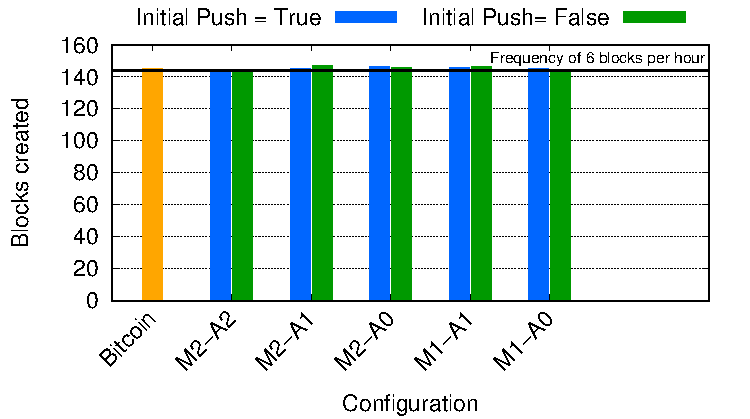
\includegraphics[width=0.45\textwidth]{plots/imp/blocks-gen.pdf}
%	\caption{Quantidade de blocos criados}
	\label{fig:nb-blocks}
}
%\end{subfigure}%
%\begin{subfigure}{.5\textwidth}
%	\centering
\subfloat[Percentagem de transações adicionadas aos blocos.]{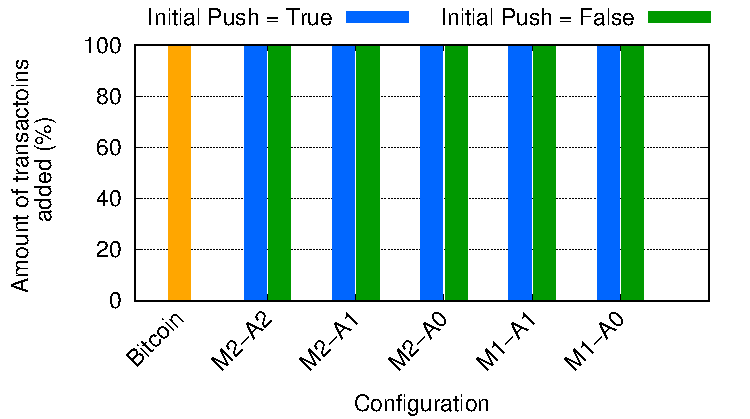
\includegraphics[width=.45\textwidth]{plots/imp/tx-added.pdf}
	\label{fig:tx-added}
}
\caption{Blocos criados e percentagem de transações adicionadas aos blocos nos diferentes cenários considerados.}
%\end{subfigure}
\vspace{-0.7cm}
\end{figure}

A Figura~\ref{fig:nb-blocks} apresenta, para cada configurações a quantidade de blocos que foi gerada ao longo da experiência, enquanto que a Figura~\ref{fig:tx-added} mostra a percentagem de transações que foram adicionadas aos blocos.
%No eixo do x temos as diferentes configurações e no eixo do y temos a percentagem de transações adicionada.
Para o cenário Bitcoin obtemos o número esperado de blocos num dia ($\approx 144$) bem como o número de transações incluídas nos blocos ($\approx 100\%$).
Todas as configurações produzem aproximadamente o mesmo número de blocos, contudo para as configurações M2\_A0 e M1\_A0 nem todas as transações são incluídas nos blocos.
Na prática isto quer dizer que nem todas as transações chegam a todos os mineiros, e ilustra a importância de manter a aleatoriedade da disseminação.

%Ambas as figuras mostram que o nosso simulador é capaz de simular com alguma fidelidade a Bitcoin pois podemos observar na coluna do Bitcoin que quantidade de blocos gerados está bastante próximo dos seis blocos à hora e que todas as transações geradas durante a simulação foram incluídas em blocos.
Na Figura~\ref{fig:commit-time} estudamos o tempo médio desde que uma transação é criada até ser incluída num bloco. As linhas horizontais denotam o tempo médio para uma transação ser incluída num bloco no Bitcoin.
%As linhas horizontais denotam o tempo médio de uma transação na coluna Bitcoin encontra-se dentro dos limites esperados.
Mais uma vez, a aleatoriedade ajuda não só a a que as transações cheguem a todos os nós como também diminui consideravelmente o tempo necessário para as transações serem incluídas nos blocos.
\vspace{-0.6cm}

\begin{figure}
\centering
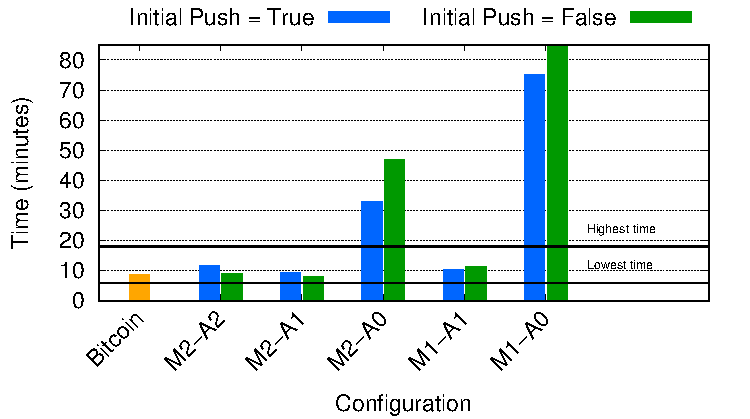
\includegraphics[width=0.8\textwidth]{plots/imp/commit-time.pdf}
\caption{Tempo médio que demora desde que uma transação é criada até ser incluída num bloco.}
%Para as configurações em que nem todas as transações são incluídas, ignoramos essas transações.}
\label{fig:commit-time}
\vspace{-1.5cm}
\end{figure}

%\subsection{Desempenho}

\begin{figure}
\centering
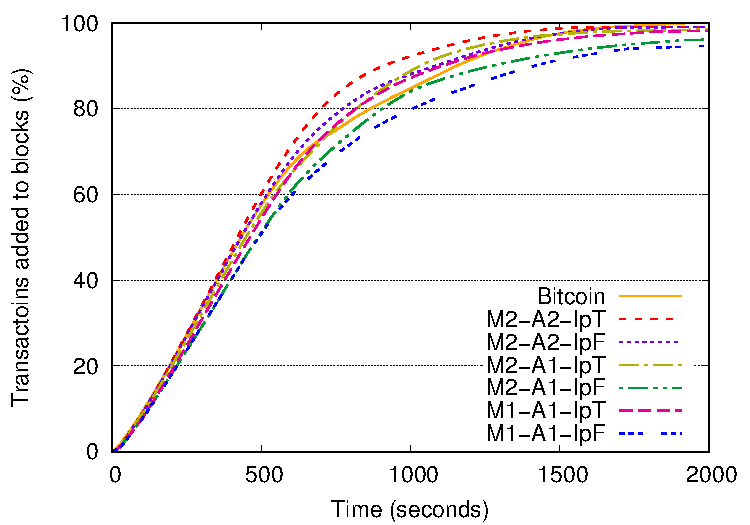
\includegraphics[width=0.6\textwidth]{plots/imp/cdf_commit.pdf}
\caption{Função de distribuição acumulada do tempo necessário para uma transação ser incluída num bloco.}
%CDF do tempo de commit. Nesta figura não mostramos no eixo do \textsl{x} todas as configurações a atingir as 100\% transações adicionadas pois se o fizéssemos a figura tornar-se-ia ilegível.}
\label{fig:cdf-commit}
\vspace{-0.5cm}
\end{figure}

A Figura~\ref{fig:cdf-commit} apresenta a função de distribuição acumulada do tempo necessário para incluir transações num bloco, sendo portanto uma perspectiva diferente da Figura~\ref{fig:commit-time}.
Curiosamente, enviar a transação a primeira vez para todos os vizinhos (\emph{pi=T}) tem um impacto residual no tempo que as transações demoram a ser incluídas no bloco.
Isto deve-se ao facto de a taxa de criação de blocos ser bastante reduzida face ao tempo de propagação fim-a-fim da rede.
%, permitindo assim poupanças adicionais.
%a CDF do tempo de commit. Nesta figura podemos observar que existem configurações onde grande parte das transações demora mais de 166 minutos a serem adicionadas aos blocos, isto acontece especialmente nas configurações M2\_A0 e M1\_ A0. Daqui conseguimos concluir que estas configurações não são muito viáveis.

\begin{figure}
\centering
\begin{minipage}{.5\textwidth}
  	\centering
  	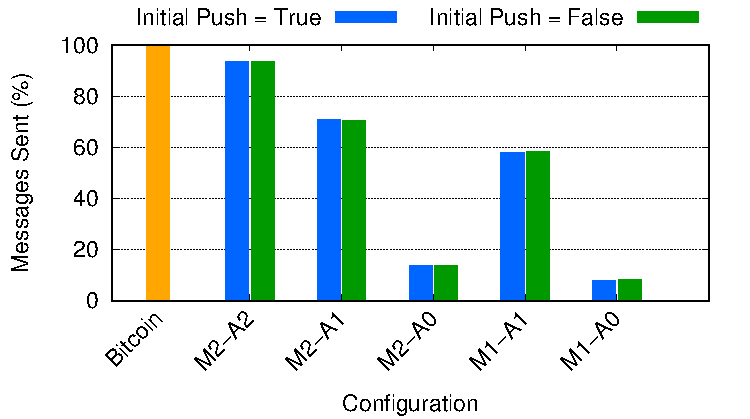
\includegraphics[width=1\textwidth]{plots/imp/msg-sent.pdf}
	\caption{Numero total de mensagens \\\hspace{\textwidth} enviadas.}
	\label{fig:msg-sent}
\end{minipage}%
\begin{minipage}{.5\textwidth}
  	\centering
  	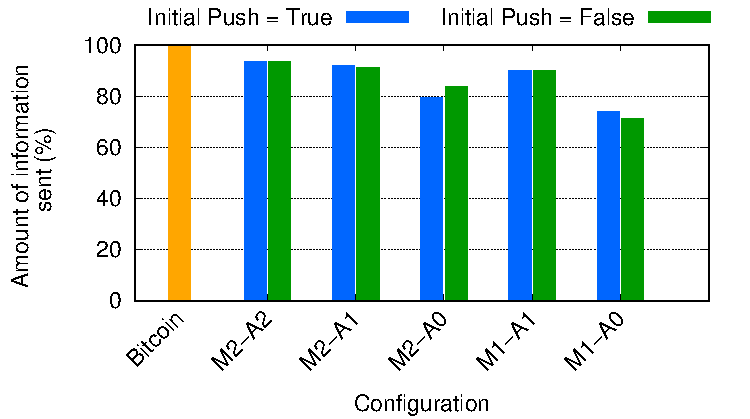
\includegraphics[width=1\textwidth]{plots/imp/mb-sent.pdf}
	\caption{Quantidade de informação \\\hspace{\textwidth} enviada.}
	\label{fig:mb-sent}
\end{minipage}
\vspace{-0.5cm}
\end{figure}

Analisado o impacto nos efeitos observáveis da rede, nomeadamente o tempo que uma transação demora a ser incluída num bloco e a quantidade de transações incluídas, focamo-nos agora no ganhos, em termos de mensagens poupadas e redução da quantidade de informação transmitida.


A Figura~\ref{fig:msg-sent} mostra o número total de mensagens que foram enviadas em percentagem das enviadas na rede Bitcoin.
%No eixo do \textit{x} temos as diferentes configurações e no eixo do \textit{y} a percentagem de mensagens enviadas em relação à versão Bitcoin.
Como esperado, as configurações com mais poupanças são as que não enviam transações para nós aleatórios, pois é provável que esses nós não tenham a transação e logo irão pedi-la ao emissor.
%isto porque ao enviar anúncios de transações para nós A vamos quase de certeza receber um pedido para a transação que anunciamos pois muito provavelmente eles ainda não têm a transação, o mesmo já não acontece quando se envia transações para nós M.
No entanto, como vimos anteriormente, estas configurações não são viáveis pois nem todas as transações são incluídas e, as que são, tendem a demorar bastante tempo.
A Figura~\ref{fig:mb-sent} mostra a quantidade de informação total enviada em percentagem que, como esperado, segue uma tendência semelhante à Figura~\ref{fig:msg-sent}.
Podemos observar que a poupança em quantidade de informação enviada não é tão significativa como a das mensagens, pois as mensagens de anúncio são pequenas.
No entanto, na prática, processar essas mensagens desnecessariamente impõe um custo nos nós.
%todos os nós vão ter sempre que acabar por receber as transações, desta forma só conseguimos poupar nos anúncios destas. No entanto entre as duas configurações de M1\_A1 podemos ver que com o push inicial a False vamos obter a maior poupança.

Analisando estes resultados, é possível concluir que a configuração mais atrativa é M1\_A1 com \textsl{pi=F} pois obtém bons ganhos
(redução da quantidade de mensagens em 40.5\% e  redução total da quantidade de informação enviada em 10.7\%) ao mesmo tempo que preserva as propriedades da Bitcoin original.
